\label{chap:dense_external_tracking}
\begin{figure}
	\begin{center}
		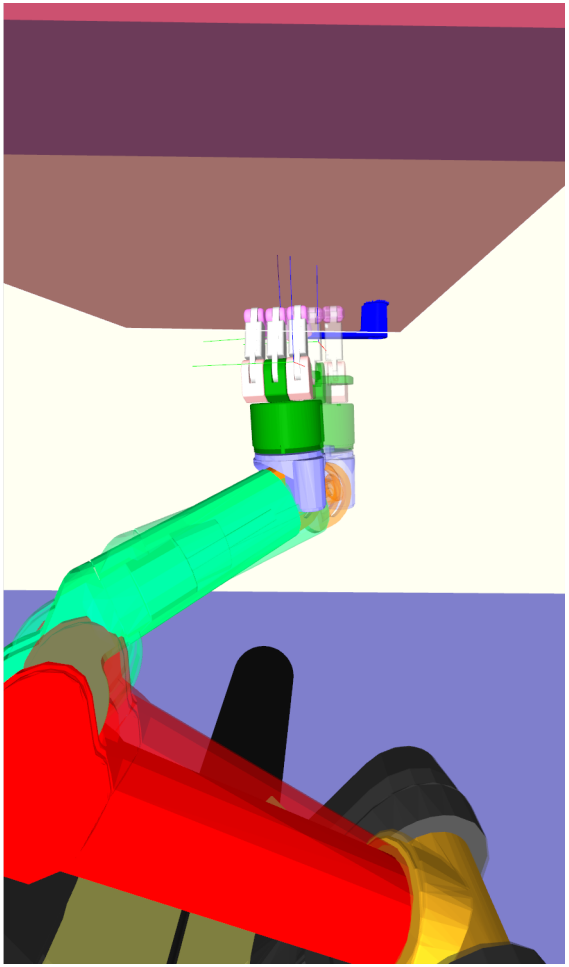
\includegraphics[width=0.24\textwidth]{img/dense_tracking/door_sim}
		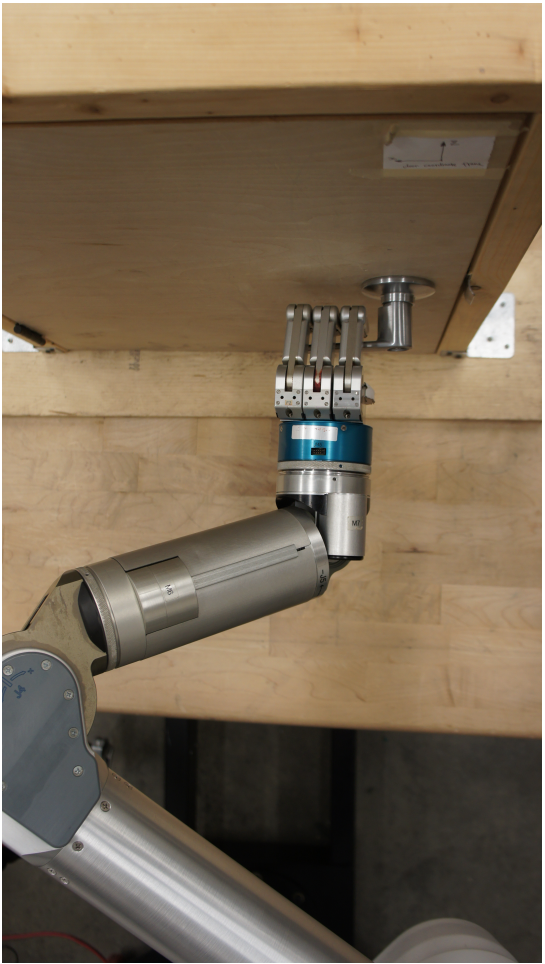
\includegraphics[width=0.23\textwidth]{img/dense_tracking/door_real}
	\end{center}
	\caption{A robot arm opens a door using dense depth tracking. Left: the robot's kinematics (solid) are compared with the estimated joint angles from the tracking system (transparent). Right: the robot is shown grasping the door handle.}
	\label{fig:door_open}
\end{figure}
\lettrine{W}e first consider the case of using an external depth camera to track a noisy robot arm in real time. In this case, a depth sensor is mounted so that it can see all or part of the robot's arm, and the robot's joint angles are estimated from the depth image. This is the simplest of the three problems we will consider, because we generally have a good 3D model of the robot arm, and this model can be used as the basis of a tracking algorithm. 

Tracking the arm in real-time also allows for a kind of 3D visual servoing, where the robot can be made to touch points in the scene while automatically correcting for its joint angle error. This rather powerful technique allows the robot to correct unforseen errors that arise from its own dynamics, contact with the scene, and more. In addition, solving this problem elucidates the structure of the related problems we will have to solve in later sections. \footnote{\textit{This chapter largely reiterates earlier work that appears in \cite{Klingensmith2013}}} 

\section{Problem Definition}
We have a series of discrete time-steps $t_1 \ldots T$ in which we receive time-synchronized measurements from the encoders $\enc_1 \ldots \enc_T$ and depth images $D_1 \ldots D_T$. How do we determine the true state of the robot from these data? One approach might be to track a rigid object on the robot's body (such as its end effector); but this ignores valuable data from other parts of the robot's body. Another approach is to track the entire robot arm using the depth image.In this section, we will derive a simple way of tracking the entire robot in \textit{configuration space} (\sref{sec:articulated_linkage}) from a series of depth images. This has several advantages: it makes full use of observations of the robot's body, it naturally constrains solutions to those which are possible given the robot's kinematics, and it provides an estimate of the joint angles which can be used for visual servoing.

The goal is to predict a maximum likelihood estimate of the robot's true configuration $\config_1 \ldots \config_T$ from these measurements. In other words, we wish to find:

\begin{equation}
	\config_T = \argmax_{\config} \Prob\left(\config | \DepthImage_1, \ldots, \DepthImage_T, \enc_1, \ldots \enc_T \right)
\end{equation}

If we model this as a Markov process, such that the state at time $T$ only depends on the state at time $T - 1$ and measurements from time $T$, and assuming conditional independence between the depth image, configuration and joint encoders we have a maximization of the log-likehihood of two terms:

\begin{align}
	\config_T &= \argmax_{\config} \Prob\left(\config | \DepthImage_T, \enc_T\right) \\
	          &= \argmax_{\config} \frac{\Prob\left(\DepthImage_T | \config\right) \Prob(\config | \enc_T)}{\Prob\left(\DepthImage_T, \enc_T\right)} \\
	          &= \argmax_{\config} \log \Prob(\DepthImage_T | \config) + \log \Prob(\config | \enc_T)
	          \label{eqn:dense_model_track}
\end{align} 

\noindent these are the depth image posterior $\Prob(\DepthImage_T | \config)$ and the joint encoder posterior $\Prob(\config | \enc_T)$. With some simple assumptions about the structure of the depth image and the joint encoders, it is possible to write these out efficiently.

\subsection{Depth Image Posterior}
From each depth image $\DepthImage_T$, produce its point-cloud $\pixel_1, \ldots, \pixel_M \in \DepthImage_T$. We assume that given the robot's configuration $\config$, the points in the point cloud correspond to some true point on the robot's body corrupted by identically distributed indepdendent random noise. Assume there is a ground-truth mapping $\beta_i(\config)$ that gives us the point on the robot's body that corresponds to the point in the point cloud of the depth image.

Assume then that the points are distributed according to a simple isotropic normal distribution so that

\begin{equation}
	\pixel_i \sim \beta_i(\pixel_i, \config) + \mathcal{N}(0, \Sigma_\pixel)
\end{equation}

\noindent where $\Sigma_\pixel =  \sigma_\pixel \eye$ is the covariance of the point cloud noise, with $\sigma_\pixel$ being the noise variance. With all these assumptions in place, the probability of seeing a particular point in the point cloud given the robot's configuration is simply

\begin{equation}
	\Prob(\pixel_i | \config) = \exp{\frac{-\|\pixel_i - \beta_i(\config)\|^2}{2 \sigma_\pixel}}
\end{equation}

\noindent and assuming conditional independence, the depth image posterior becomes

\begin{equation}
	\Prob(\DepthImage_T | \config) = \prod_{\pixel_i \in \DepthImage_T} \Prob(\pixel_i | \config)
\end{equation}

\noindent and finally the log-likelihood becomes

\begin{equation}
	\log \Prob(\DepthImage_T | \config) = -\frac{1}{2 \sigma_\pixel}\sum_{\pixel_i \in \DepthImage_T} \| \pixel - \beta_i(\config) \|^2
\end{equation}

Computing the posterior requires associating each point in the point cloud with a point on the robot's body. If these associations are unknown, we can use physical distance as a heuristic to match a point in the point cloud to one on the robot's body. That is:

\begin{equation}
	\bar{\beta_i}(\config) = \argmin_{\beta \in \mathbf{B}(\config)} \|\beta - \pixel_i\|
\end{equation}

\noindent where $\mathbf{B}(\config)$ is the set of all points on the robot's body while the robot is in configuration $\config$ that can be viewed by the depth camera (and which are not self-occluded). This heuristic is similar to the one used in the Iterative Closest Point (ICP) algorithm. Because we use every pixel in the depth image, this is a \textit{dense} tracking technique (as opposed to a technique which only uses sparse image features).

\subsection{Joint Encoder Posterior}
The relationship between the joint encoders $\enc$ and actual configuration $\config$ of the robot might be quite complicated; but here we use a very simple model of the joint encoder noise that is sufficient to capture it. Assume we have a fixed calibration $K_\enc(\enc)$ which converts joint encoders to robot configurations (\sref{sec:encoders}), and assume that the true robot configuration is drawn from an isotropic gaussian distribution around this function. That is:

\begin{equation}
	\config_T \sim K_\enc(\enc_T) + \mathcal{N}(0, \Sigma_\config)
\end{equation}

\noindent where $\Sigma_\config = \sigma_\config \eye$, and  $\sigma_\config$ is the isotropic variance of the noise. With these assumptions, we can write the joint encoder posterior as

\begin{equation}
	\Prob(\config_T | \enc_T) = \exp{-\frac{\|K_\enc(\enc_T) - \config\|^2}{2 \sigma_\config}}
\end{equation} 

\noindent and the log-likelihood is simply

\begin{equation}
	\log P(\config_T | \enc_T) = -\frac{\|K_\enc(\enc_T) - \config\|^2}{2 \sigma_\config}
\end{equation}

\noindent admittedly, this model of joint encoder noise is not completely accurate, as it assumes there is time-independent random noise on the joint-encoders, when in reality there are likely to be systematic biases that depend on the configuration of the robot, time, or both. We will explore more complex posteriors in later sections.

\section{Algorithm Implementation}
We implement the algorithm using stochastic gradient ascent of the log-likelihood function. The algorithm can be summarized as follows:

\begin{enumerate}
  \item Synchronize depth images and joint encoders at time $T$ to produce $\DepthImage_T$ and $\enc_T$.
  \item Initialize the gradient descent using the mode of the joint encoder posterior $\config_{k} = K_\enc(\enc_T)$.
  \item Render the robot's body in the depth image frame at time $T$ to produce a set of body points $\mathbf{B}(\config_{k})$
  \item Match each body point to its nearest neighbor in the point cloud to calculate an estimate of $\Prob(\DepthImage | \config_{k})$
  \item Minimize the negative log-likelihood using stochastic gradient descent.
  \item Repeat.
\end{enumerate}

\begin{figure}[ht]
	\centering
	\begin{subfigure}{0.45\textwidth}
		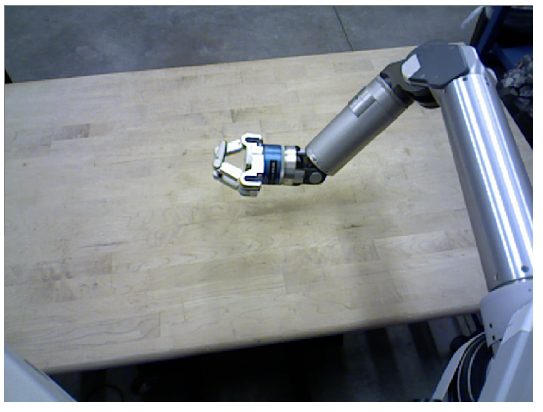
\includegraphics[width=1.0\textwidth]{img/dense_tracking/rgb_input}
		\caption{RGB input (not used)}
	\end{subfigure}
	\begin{subfigure}{0.45\textwidth}
		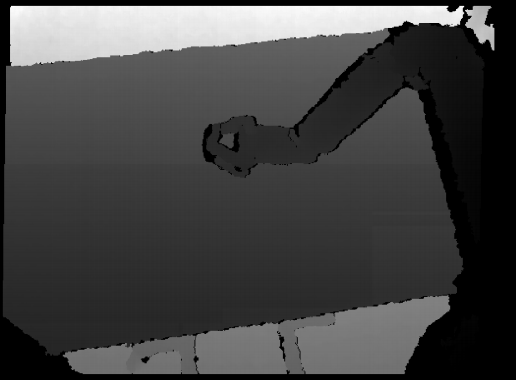
\includegraphics[width=1.0\textwidth]{img/dense_tracking/depth_input}
		\caption{Depth input}
	\end{subfigure}
	\begin{subfigure}{0.45\textwidth}
		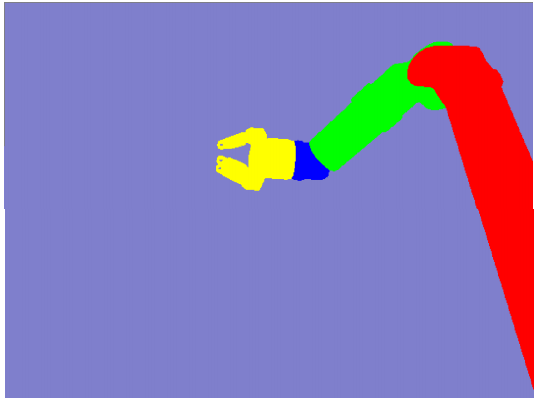
\includegraphics[width=1.0\textwidth]{img/dense_tracking/label_render}
		\caption{Synthetic label image}
	\end{subfigure}
	\begin{subfigure}{0.45\textwidth}
		\centering
		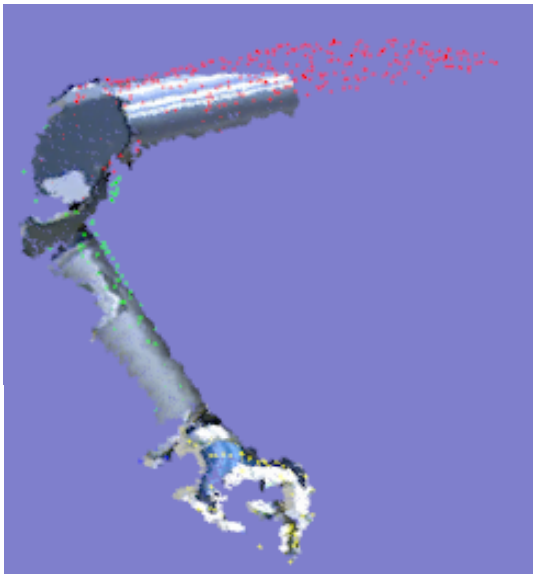
\includegraphics[width=0.75\textwidth]{img/dense_tracking/pointclouds}
		\caption{Synthetic and real point clouds}
	\end{subfigure}
	\caption{Images taken during different phases of the dense tracking algorithm.}
    \label{fig:dense_tracking}
\end{figure}

\subsection{Matching to the depth image}
Our implementation relies on quickly rendering and matching points of the robot's body to points in the point cloud. To achieve this, we render a \textit{synthetic point cloud} (\figref{fig:dense_tracking}) using a CAD model of the robot and the depth camera's intrinsics. Points are labeled by the GPU according to the link they are associated with. Each synthetic point is then matched to a real point in the point cloud using an octree. Outliers are rejected. The result is a conservative matching between the synthetic point cloud and the real one which naturally handles occlusion and segmentation.

\subsection{Stochastic gradient descent}
We compute the stochastic gradient of the log-likelihood function with respect to the robot's configuration by randomly sampling $M$ points of the robot's body and computing:

\begin{align}
	\frac{\partial}{\partial \config} \log \Prob(\DepthImage | \config) &\approx \sum_{i = 1}^{M}  \frac{\partial}{\partial \config}  \Prob(\pixel_i | \config) \\
		&= -\frac{1}{\sigma_\pixel}\sum_{i = 1}^{M} \J_{\beta_i}\trans\left(\pixel - \beta_i(\config)\right)
\end{align}

\noindent where $\J_{\beta_i}$ is the linear kinematic Jacobian of the robot arm evaluated for body point $\beta_i$ (\sref{sec:kinematics}). The gradient of the joint encoder posterior can also be computed as

\begin{align}
	\frac{\partial}{\partial \config} \log \Prob(\config | \enc) = -\frac{K_\enc(\enc_T) - \config}{\sigma_\config}
\end{align}

We use the stochastic gradient, rather than the full gradient, to save on computation. The gradient descent step is then:

\begin{equation}
	\config^{(k +1)} = \config^{(k)} - \lambda\left(\frac{\partial}{\partial \config} \log \Prob(\config | \enc) + \frac{\partial}{\partial \config} \log \Prob(\DepthImage | \config)\right)
\end{equation}

\noindent where $\lambda$ is a learning rate. We repeat until $\config^{(k)}$ converges, and becomes the new estimated state of the robot's joint angles.

\section{Experiments}

We tested the dense tracking algorithm on the DARPA ARM-S robot, which has an Asus \textit{Xtion Pro} depth sensor and a Barret WAM arm. Timing data for the tracker is shown in \tableref{tab:dense_track_time}. On average, the tracker runs at more than $100$ Hz (the majority of time being spent creating the synthetic point cloud image and shuffling data back and forth between the GPU). This is fast enough to incorporate into a real-time control loop for visual servoing.

\begin{table}
\centering
\begin{tabular} {l|l}
    Algorithm Step     & Average time per frame (ms) \\
    \hline
	Forward Kinematics & 0.1 \\
	Gradient Calculation & 0.2  \\
	Data Association & 1.5  \\
	Synthetic Rendering & 8.0
\end{tabular}
\caption{Timing data for the dense tracking algorithm. Notice that rendering the synthetic point cloud takes up the vast majority of the time. Altogether, the algorithm runs at $\sim100$ Hz.}
\label{tab:dense_track_time}
\end{table}

To verify that the algorithm was really reducing error in the robot's joint angles, we conducted an experiment where the robot was asked to touch a 2cm radius red dot repeatedly from different directions with randomly sampled inverse kinematics solutions. The red dot was detected using HSV blob segmentation in the RGB-D image, and its centroid in the point cloud was treated as the 3D target that the robot was to servo toward (\figref{fig:touching_track}). We measured how far the finger tip fell from the center of the red dot as a measure of accuracy. The experiment was performed 15 times for each case (with and without dense tracking), using the same randomly sampled starting end ending configurations for the arm.

\begin{figure}[width=1.0\textwidth]
\centering
\begin{subfigure}{0.4\textwidth}
	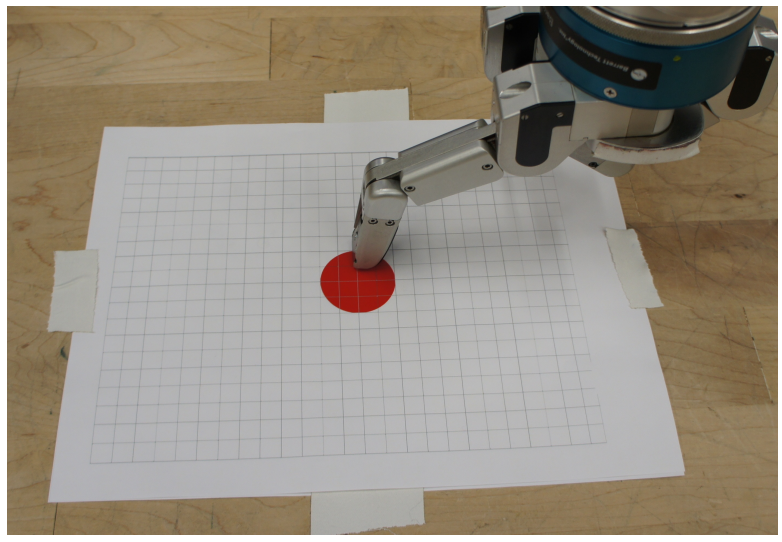
\includegraphics[width=1.0\textwidth]{img/dense_tracking/track_touch}
	\caption{}
\end{subfigure}
\begin{subfigure}{0.4\textwidth}
	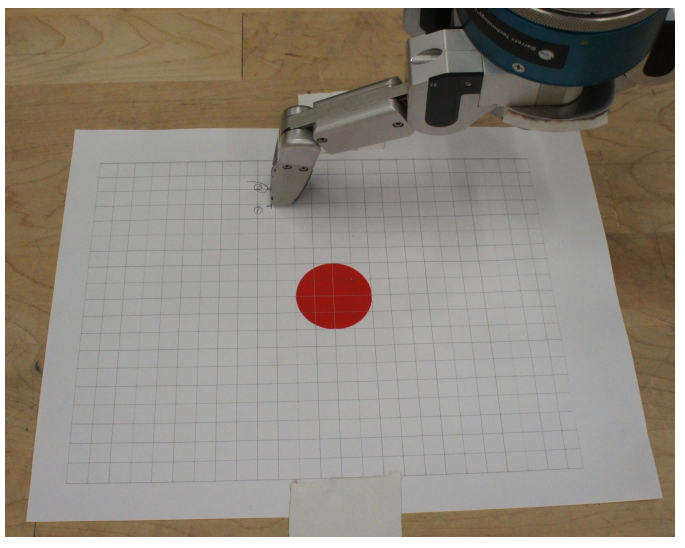
\includegraphics[width=0.9\textwidth]{img/dense_tracking/openloop_touch}
	\caption{}
\end{subfigure}
	\begin{subfigure}{0.5\textwidth}
	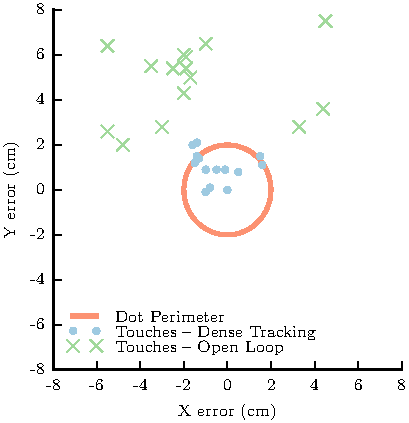
\includegraphics[width=0.9\textwidth]{img/dense_tracking/dots}
	\caption{}
	\label{fig:touching_data}
	\end{subfigure} 
\caption{The visual servoing experiment. Left: the robot servos toward the red dot while tracking its joint angles with the depth image. Right: the robot servos toward the red dot without tracking its joint angles with the depth image.}
\label{fig:touching_track}
\end{figure}

\figref{fig:touching_data} shows the error of the fingertip when using visual servoing and without. Tracking the arm in the depth image resulted in error that was well under 2cm, while using open-loop position control resulted in errors that were in excess of 7cm. 

This kind of error reduction allows us to perform more precise manipulation tasks. Figure \figref{fig:door_open} shows an example of such a task: the robot uses dense tracking to servo toward a door handle and open it. We performed this experiment 10 times. The robot was said to succeed whenever its fingers caged the door handle, and was said to fail whenever its fingers missed the door handle completely, collided with the door, or hit the door handle and slipped off. With visual servoing from dense arm tracking, the robot succeeded 9/10 times. With open-loop position control, the robot succeeded 0/10 times.

\section{Discussion and Limitations}
We have shown an example of how visual data can be used to correct joint angle uncertainty for a robot arm, and how this correction can be used to improve the robot's performance. The key idea behind this simple algorithm involves treating the problem as one of maximum likelihood estimation in the configuration space of the robot, given the sensor data.

However, this algorithm has severe limitations. First, it assumes all of the error comes from joint angle offsets along the axis of the robot's joints. It treats this uncertainty as simple isometric Gaussian noise on the joint encoders, when in reality the noise is likely to be nonlinear and depends on factors such as gravity and torque. 

The technique fails to explicitly estimate the uncertainty of the robot arm's state. Rather, it just estimates a single maximum-likelihood estimate. Because it makes the Markov assumption, the dense tracker does not make use of the entire robot trajectory to estimate the state. This makes the technique prone to local minima.

Because we use simple point-to-point data associations between the robot's body and the depth image, we run the risk of mismatching data. Because we rely on simple gradient descent to optimize the log-likelihood function, the algorithm is not very robust to outliers caused by mis-matching of data. This will occur if any un-modeled objects (such as objects held in the robots hand, or surfaces occluding the arm) are visible in the depth image near the arm.

Finally, this technique relies on a depth camera that can see all or part of the robot's arm. What do we do if the camera is mounted on the robot's hand (and hence can't see any part of the robot's arm)? What if depth is not available? We will tackle some of these problems in the next two chapters.